\documentclass{standalone}

\usepackage{pgf,tikz}
\usetikzlibrary{calc,shapes,backgrounds,arrows,automata,shadows,positioning}
\definecolor{myorange}{HTML}{FAB20A}
\definecolor{myblue}{HTML}{0000FF}
\definecolor{mygreen}{HTML}{008000}

\begin{document}

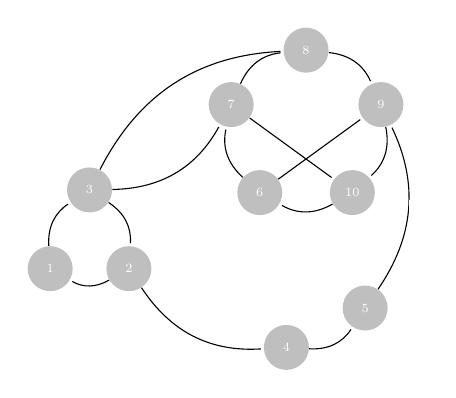
\begin{tikzpicture}
  %% UN GRAPH

  \tikzstyle{every edge}=[-,>=stealth',shorten >=1pt,auto,thin,draw]
  \tikzstyle{every state}=[draw=none,text=white,scale=0.65, font=\scriptsize, transform shape]
  \tikzstyle{every node}=[fill=lightgray]
  % premier cluster
  \node[state] (A1) at (0,0.5) {1};
  \node[state] (A2) at (1,0.5) {2};
  \node[state] (A3) at (.5,1.5) {3};

  \path (A2) edge [bend left] node[fill=white,below=.1cm]
  {}
  (A1)
  (A1) edge [bend left] (A3)
  (A3) edge [bend left] (A2);

  \tikzstyle{every node}=[fill=blue!80!black]
  \foreach \angle/\text in {234/6, 162/7, 90/8, 18/9, -54/10} {
    \node[fill=lightgray,state,xshift=5cm,yshift=3.5cm]     (\text)    at
    (\angle:1cm) {\text};
  }
  \path (7) edge (10)
  (6) edge (9);
  \foreach \from/\to in {6/7,7/8,9/10,10/6}{
    \path (\from) edge [bend left] (\to);
  }

  \path    (8)    edge     [bend    left]    node[fill=white]
  {}  (9) ;

  \tikzstyle{every node}=[fill=lightgray]
  % troisieme cluster
  \node[state] (C1) at (3,-.5) {4};
  \node[state] (C2) at (4,0) {5};

  \path (C1) edge [bend right] (C2);

  % inter cluster
  \path (A3) edge [bend right]  (7)
  (A3)    edge    [bend    left]    node[fill=white]
  {}
  (8)
  (C2) edge [bend right] node[fill=white,right]
  {}
  (9)
  (A2) edge [bend right] node[fill=white]
  {}
  (C1);
\end{tikzpicture}
\end{document}
